\chapter{Anwendungen der KI}
\label{chap:Anwendungen}

\section{KI-Anwendungen}
Die KI ist nicht mehr wegzudenken, da sie bereits heute in vielen Bereichen unseres Alltags präsent ist. Wer nur an Chat Gpt denkt, liegt hier komplett falsch. Oft kommen wir in Berührung mit der KI, ohne es wirklich wahrzunehmen. Ob Schachspiel gegen einen Computer, Besuch eines Online Shops, Interaktion mit Sprachassistenten oder Verwendung eines Übersetzungsdienstes. In all diesen Situationen kommen wir in Kontakt mit der Künstlichen Intelligenz. Von einer Schwachen KI spricht man, wenn die KI auf den Bereich beschränkt ist, indem sie eingesetzt wird, also nur in einem spezifischen Bereich ziemlich gut ist. Dies ist heutzutage in den meisten Situationen der Fall, da es "noch" keine starke KI gibt, die das menschliche Gehirn übertrifft und auf verschiedenen Bereichen verwendet werden kann. 

\begin{figure}[h]
    \centering
    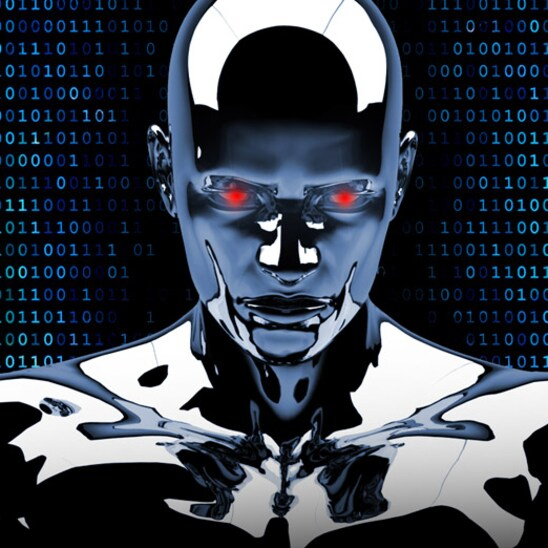
\includegraphics[width=0.5\textwidth]{AI1.jpg} 
    \caption{Gefahren der KI}
    \label{fig:ai}
\end{figure}

\section{Kann die KI gefährlich werden?}
Die KI, der grosse technologische Fortschritt der heutigen Zeit, ihre  Entwicklung  schreitet rasch voran und die Einsatzmöglichkeiten nehmen zu. Neben den vielen Vorteilen, besteht auch eine Gefahr, dass die KI eines Tages schlauer wird als Menschen. Steht also wirklich das Verderben der Menschheit durch die KI vor? Kann die KI aber tatsächlich Arbeitskräfte ersetzen? Die KI, ein Segen oder doch ein Fluch? Die KI wird in der Zukunft den Arbeitsalltag vieler Menschen ändern. Studien zeigen, dass Berufe wie z.B Mathematiker oder Programmierer am meisten bedroht sind. Das muss jedoch nicht unbedingt heissen, dass viele Arbeitskräfte ihren Beruf nicht mehr ausführen können, sondern dass sie von lästigen Aufgaben entlastet werden und mehr Zeit haben für Tätigkeiten, bei denen man nicht auf Menschen verzichten kann. Die KI kann zum Beispiel viele Bereiche der Medizin revolutionieren. Die Themen Rassismus und Sexismus kommen im Bereich der KI leider nicht selten vor, da KI- Systeme wie z.B Chat Bots aus Daten lernen, welche häufig nicht neutral sind, wiederspiegelt das System dies und kann diskriminierende Entscheidungen treffen. In den letzten Wochen und Monaten haben Nachrichten über Deep Fakes durch AI zugenommen. Die Künstliche Intelligenz erlaubt es uns Fotos, Videos als auch Audiodateien zu manipulieren. Viele Stars und Politiker wurdern bereits Opfer von den sogenannten Deep Fakes. All diese Szenarien zeigen, dass wir sehr verantwortungsbewusst mit der KI umgehen müssen und ihre Einsatzmöglichkeiten wie z.B das Erstellen von Deep Fakes beschränken müssen. Jedoch will ich noch betonen, dass sich hinter der KI einige Gefahren verbergen, aber auch sehr viele positive Aspekte. In den sozialen Medien wird die Gefahr der KI übertrieben dargestellt, was eher einer unrealistischen Fiktion entspricht

